\documentclass{scrartcl}
\usepackage{german}
\usepackage[T1]{fontenc}
\usepackage[latin1]{inputenc}
\usepackage[german]{babel}

% zusätzliche mathematische Symbole, AMS=American Mathematical Society
\usepackage{amssymb}

% fürs Einbinden von Graphiken
\usepackage{graphicx}

% für Namen etc. in Kopf- oder Fußzeile
\usepackage{fancyhdr}

% erlaubt benutzerdefinierte Kopfzeilen
\pagestyle{fancy}

% Definition der Kopfzeile
\lhead{
\begin{tabular}{ll}
Fisnik Zeqiri & 4306430 \\
Felix  Karg   & 4342014
\end{tabular}
}
\chead{}
\rhead{\today{}}
\lfoot{}
\cfoot{Seite \thepage}
\rfoot{}

\begin{document}
\section*{Antworten zum �bungsblatt Nr. 11}

\section*{Aufgabe 1}
    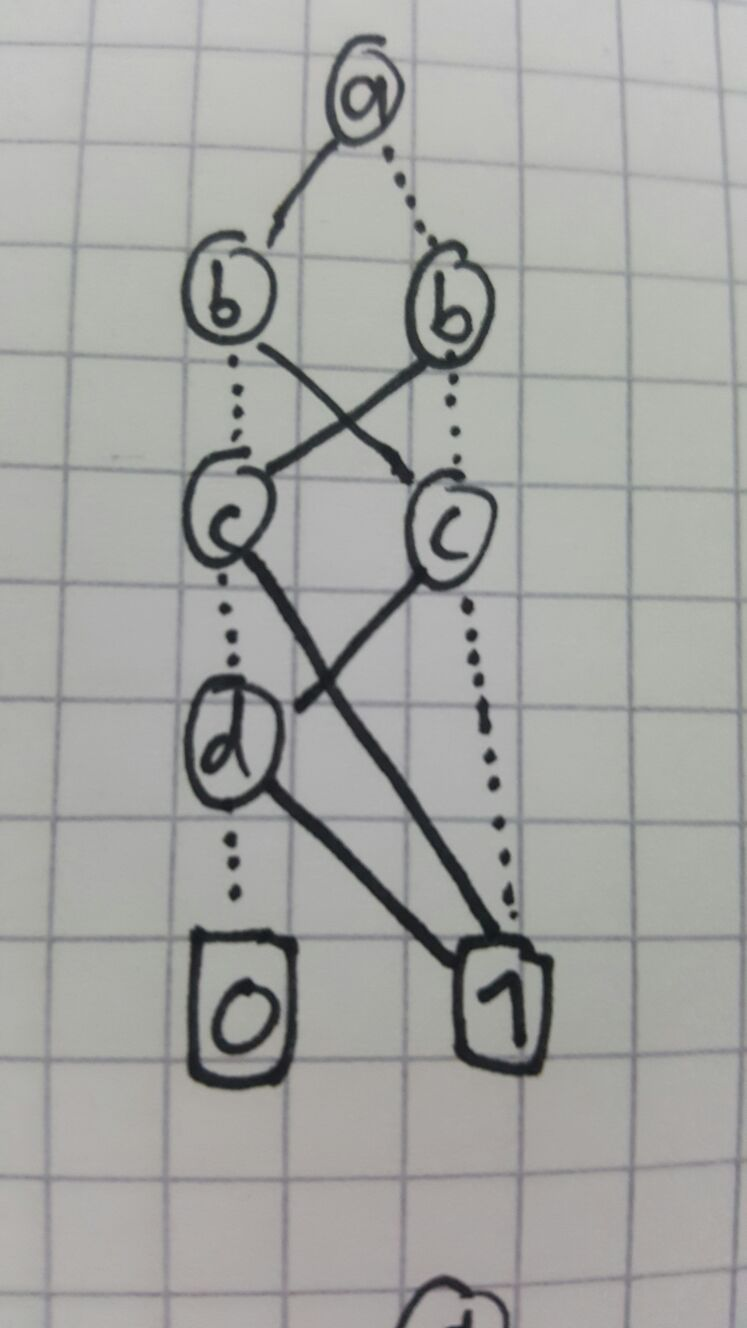
\includegraphics[width=9cm]{1.jpg}
\begin{itemize}
%    \item DNF: $a'bc+ab'c+abc'+a'b'c'+d$
    \item DNF: $(a' \wedge b \wedge c) \vee (a \wedge b \wedge 'c) \vee (a \wedge b \wedge c')
        \vee (a' \wedge b' \wedge c') \vee d$
    \item KNF: $((a \vee b' \vee c') \wedge (a' \vee b \vee c') \wedge (a' \vee b' \vee c)
        \wedge (a \vee b \vee c) \wedge d')' $
\end{itemize}

\section*{Aufgabe 2}
a) \\
Bedingend durch die Existenz neutraler Elemente (Axiom) sowie die Idempotenz (Herleitbar) ist
offensichtlich dass es entweder ein Element gibt dass gleichzeitig das 0- sowie das 1-Element ist,
welches gleichzeitig sein eigenes Komplement sein m�sste (dann w�ren an sich alle Axiome erf�llt),
da es allerdings ein weiteres (ungleiches !) Element gibt, lassen sich Konjunktion, Disjunktion
und das Komplement offensichtlicherweise nur dann sinnvoll definieren, wenn eines Davon zumindest
�quivalent der 1 ist, und das andere das entsprechende Komplement (also 0) ist.  \hfill $\Box$ \\

b) \\
Beh.: Es ist (in einer Booleschen Algebra) nicht m�glich, dass ein Element das Komplement seiner
selbst ist. \\
Bew.: Angenommen es gibt so ein Element a. Dann ist laut der Eindeutigkeit des Komplements
(herleitbar) sowohl $a*(~a)=a*a=1$ als auch $a+(~a)=a+a=0$, womit laut Idempotenz (Axiom) $a$ also
gleichzeitig $a = 0$ als auch $a = 1$ sein m�sste, Widerspruch! Es kann also kein Element das
Komplement seiner selbst sein. \\

In einer Boole'schen Algebra muss es zu jedem Element ein Komplement geben. Addition sowie
Multiplikation (in unserem Fall Disjunktion und Konjunktion) lassen sich auch f�r Drei-Elementrige
K�rper sinnvoll definieren (Beweis: entweder bekannt oder �bung!), allerdings nicht Negation.
Da unser neues Element $a$ ungleich $1$ und ungleich $0$ ist, muss auch das Komplement ungleich
der beiden sein (Doppelte Negation), da wir allerdings nur dieses Dritte Element ('zur Verf�gung')
haben, m�sste es sein eigenes Komplement sein, welches wir bereits bewiesen haben dass es in einer
Boole'schen Algebra nicht m�glich ist! \hfill $\Box$

\section*{Aufgabe 3}
\begin{itemize}
    \item[a)]
        $f_{x2}= x_1 $ \\
        $f_{x_3.1} = x_1' + x_2' $ \\
        $f_{x3.2} = x_1x_2 $ \\
        $f_{x4} = x_1'x_3 + x_1x_2'x_3 $ \\
        $f_{x5} = x_1'x_3x_4' + x_1x_2'x_3x_4'$ \\
        $f_{on} = f_{x3}*x_3' + f_{x3}*x_3 + f_{x4}*x_4 + f_{x5}*x_5 $ \\
        $f_{on} = x_1'x_3x_4 + x_1'x_3x_4'x_5 + x_1x_2x_3 + x_1x_2x_3' $
            $ + x_1x_2'x_3x_4 + x_1x_2'x_3x_4'x_5$
    \item[b)] Das BDD ist geordnet, jedoch nicht reduziert. wenn $x_1=x_2=1$ sind,
        ist es egal was $x_3$ ist. \\
    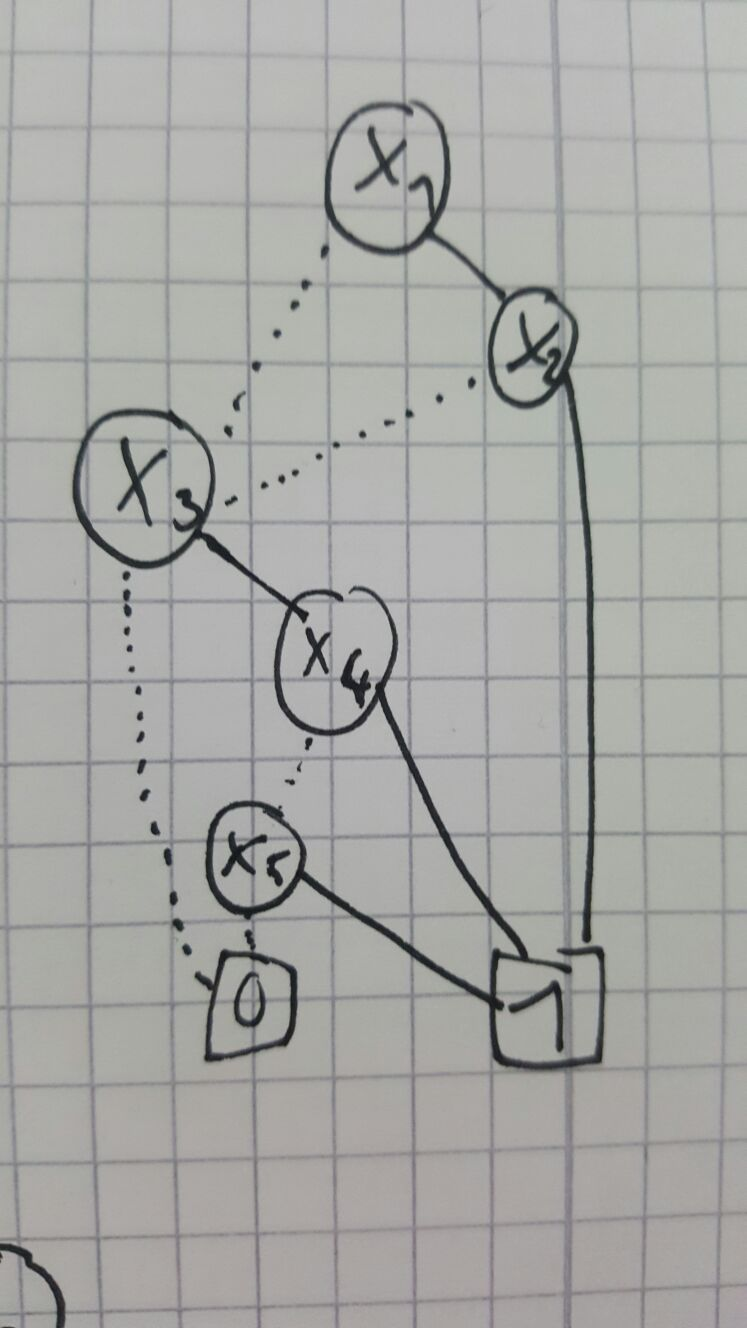
\includegraphics[width=8cm]{3.jpg}
\end{itemize}


\section*{Aufgabe 4}
Beh.: Zu jedem Boole'schen Ausdruck $e \in BE(X_n)$ existiert ein Schaltkreis $SK_e$, der e
berechnet. \\ \\
Bew.: Induktion �ber Boole'sche Ausdr�cke und Schaltkreise. \\
Boole'sche Algebra: $(M, 0, 1, \vee, \wedge, ^c)$ \\
IA: Die Elemente 0 und 1 lassen sich einfach als SK darstellen, man verbindet einfach
GND bzw. VCC mit dem Ausgang. \\
IV: F�r die Boole'schen Ausdr�cke $a$, $b$ gibt es bereits Schaltkreise $c$, $d$ die diese Berechnen. \\
IS: Dann gibt es auch Schaltreise f�r die Ausdr�cke $a^c$, $a \vee b$, $a \wedge b$.
Bew.: Um $a^c$ zu berechnen, also das Komplement von $a$, nehmen wir den $a$-Berchnenden SK $c$ und
negieren das Ergebnis dessen ($not c$). \\
Um nun $a \vee b$ bzw. $a \wedge b$ zu berechnen, Nehmen wir die Ergebnisse der SK $c$, $d$, und
Ver-Odern bzw. Ver-Unden die Ergebnisse, Fertig. \hfill $\Box$


\section*{Aufgabe 5}
ZZ:  \\
Absorption:  $x + (x *  y) = x$   $x * (x +  y) = x$ \\
Komplement:  $x + (y * ~y) = x$   $x * (y + ~y) = x$ \\
F�r Boole'sche Potenzmengenalgebra Pot(A). \\ \\
Bekannt: x und y sind jeweils Mengen, $\cup = \vee$, $\cap = \wedge$. \\ \\
Absorption: $x + (x *  y) = x \sim x \cup (x \cap y) = x$. \\
Der schnitt zwischen x und y ist Zwingend eine Menge kleiner x, wessen Elemente aber 
zwingend in x enthalten sein m�ssen (Schnitt). Die Vereinigung mit x ist also eine 
Vereinigung von x mit Elementen die zwingend schon in x 
enthalten sein m�ssen (oder der leeren Menge, aber dann ist die Vereinigung auch x). \\ \\
Absorption $x * (x + y) = x \sim x \cap (x \cup y) = x$. \\
Hier wird x mit y Vereinigt, was eine Menge gibt die vermutlich gr��er x ist, allerdings
wird danach wieder mit x geschnitten. Es sollte offensichtlich sein, dass hier nun wieder
x das ergebnis ist, da x Geschnitten mit einer Menge die x und mehr Elemente enth�lt,
wieder nur x ist. \\ \\
Komplement: $x + (y * \sim y) = x \sim x \cup (y \cap y^c) = x$. \\
y geschnitten mit dem Komplement seiner selbst, also die Ganze Menge ohne y ist gezwungenerma�en
die Leere Menge, da in der Negation von y alle Elemente enthalten sind, die nicht in y enthalten
sind. x Vereinigt mit der Leeren Menge ist offensichtlicherweise wieder x. \\ \\
Komplement: $x * (y + \sim y) = x \sim x \cap (y \cup y^c) = x$. \\
y Vereinigt mit seinem Komplement ist bekannterweise die Ganze Menge, und x Geschnitten mit der
Ganzen Menge ist trivialerweise wieder x.




\end{document}

